%% Briefly discuss the website and some of its main components.

\todo{make sure to focus on vulnerabilities}
Our website has several primary components for different users. For more technical users and researchers, we have provided a SQLite database containing application, commit, and static analysis results for each application. This database can be easily downloaded for offline research. As shown in Figure~\ref{fig:webpagequery}, users may also explore the data by writing their own queries against the dataset right on the webpage.

\begin{figure}[ht!]
\centering
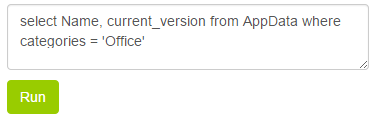
\includegraphics[width=\columnwidth, angle = 0, scale=.8]{images/webpageQuery.png}
\caption{Webpage Search Query}
\label{fig:webpagequery}
\end{figure}



%% Wifi-Automatic's google play website says that it needs the permission we have being deemed as being over prived. I am not sure if this is a problem or not.

%%% Much of this copied from the MSR paper\
Researchers and more casual users may use various default reports available on the website. A user can use the web portal and  search  for information about a specific app, snapshot of this search is shown in Figure~\ref{fig:appsearch}. We provide data about individual app versions as collected from static analysis including over and under permissions, Androrisk vulnerability scores, defect analysis, and code complexity. As an example, we will provide information about~\emph{Wifi-Automatic}\cite{wifi_automatic_GH}, a popular app with over 100,000 installs from GooglePlay. This app automatically disables a phone's wifi in order to save battery life. Figure~\ref{fig:specificAppInfo} shows defect information about the app over the course of multiple versions. In this example, the first two versions of the app had two over-privileges, while the most recent version only had one, while all versions had a single recorded underprivilege.




\begin{figure}[ht!]
\centering
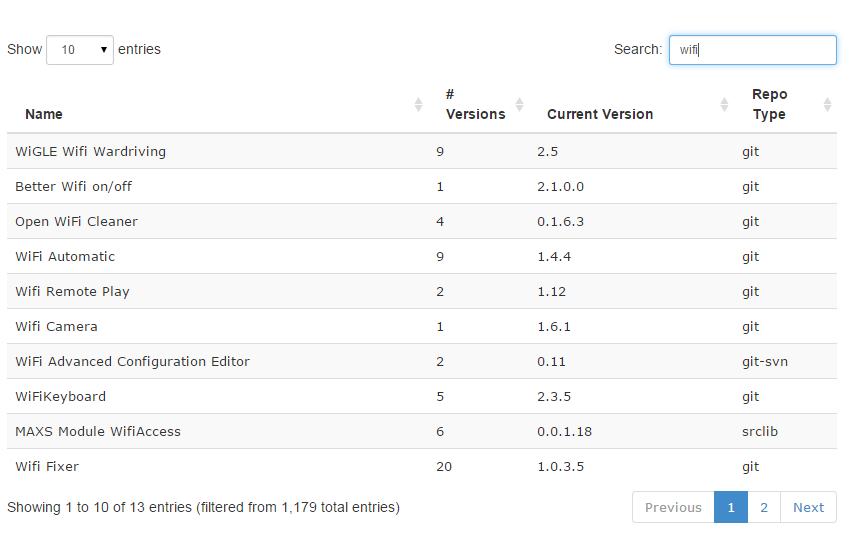
\includegraphics[width=\columnwidth, angle = 0]{images/wifi-automatic_app_search.png}
\caption{App Search for ``Wifi-Automatic'' }
\label{fig:appsearch}
\end{figure}

\begin{figure}[ht!]
\centering
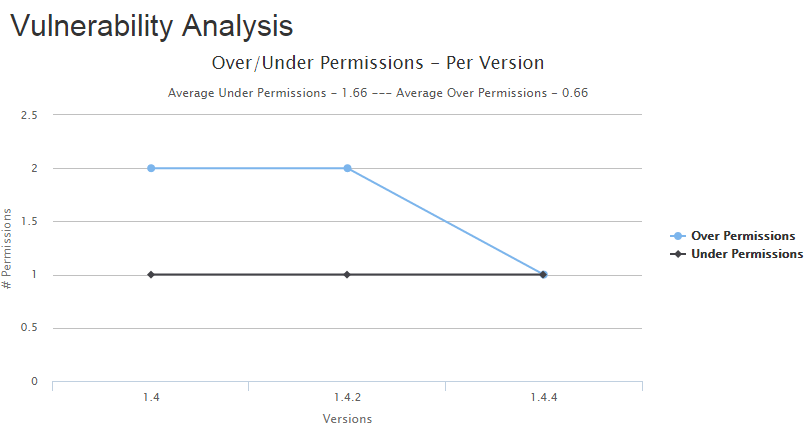
\includegraphics[width=\columnwidth, angle = 0]{images/wifi-automatic-oprivs.png}
\caption{Overprivileges for ``Wifi-Automatic'' App}
\label{fig:specificAppInfo}
\end{figure}


The website also contains several built in analytics such reports showing Androrisk, over permission rate, and coding violations rate by genre. Similar information is also shown for the most popular apps.

%%% Specific Apps


%190 - 100,000 installs
%963
%85
%176
%436
%473
%474
%843 - no downloads
    %wifi automatic % 190

    %FTP Server (Demo) - 383

    %UberSync for Facebook - 963 - Pretty good
    %XBMC Remote - 144 - not good
    %Document Viewer - 495

%Beam File - 85
%FrostWire - 176
%BetterBatteryStats - 189
%Android Tipitaka - 436
%Open Explorer Beta - 473
%F-Droid - 474
%G2L - 612
%YAACC - 765 - Good for over and under privs
%Lightning - 843

